\documentclass[aspectratio=169, 10pt]{beamer}

% Color definitions
\definecolor{Garnet}{HTML}{73000A}
\definecolor{GarnetDark}{HTML}{500007}
\definecolor{Rose}{HTML}{CC2E40}
\definecolor{Atlantic}{HTML}{466A9F}
\definecolor{Congaree}{HTML}{1F414D}
\definecolor{Horseshoe}{HTML}{65780B}
\definecolor{Grass}{HTML}{CED318}
\definecolor{Honeycomb}{HTML}{A49137}
\definecolor{Black90}{HTML}{363636}
\definecolor{Black70}{HTML}{5C5C5C}
\definecolor{Black50}{HTML}{A2A2A2}
\definecolor{Black30}{HTML}{C7C7C7}
\definecolor{Black10}{HTML}{ECECEC}

% Packages
\usepackage{amsmath,amssymb}
\usepackage{tikz}
\usetikzlibrary{arrows.meta,positioning,shapes.geometric,fit,calc}
\usepackage{pgfplots}
\pgfplotsset{compat=1.18}
\usepackage{graphicx}
\usepackage{algorithm}
\usepackage{algorithmic}

% Theme configuration
\usetheme{default}
\usecolortheme{default}
\setbeamertemplate{navigation symbols}{}
\setbeamertemplate{blocks}[default]
\setbeamertemplate{itemize items}[square]

% Colors
\setbeamercolor{structure}{fg=Garnet}
\setbeamercolor{frametitle}{bg=Garnet,fg=white}
\setbeamercolor{title}{bg=Garnet,fg=white}
\setbeamercolor{alerted text}{fg=Rose}
\setbeamercolor{block title}{bg=Atlantic,fg=white}
\setbeamercolor{block body}{bg=Black10,fg=Black90}

% Frame title template - sharp edges
\setbeamertemplate{frametitle}{
    \nointerlineskip
    \begin{beamercolorbox}[wd=\paperwidth,ht=0.8cm,dp=0.3cm]{frametitle}
        \hspace{0.5cm}\strut\insertframetitle\strut
    \end{beamercolorbox}
}

% Footer
\setbeamertemplate{footline}{
    \leavevmode%
    \hbox{%
    \begin{beamercolorbox}[wd=.333333\paperwidth,ht=2.5ex,dp=1ex,left]{author in head/foot}%
        \hspace{0.3cm}\scriptsize AIAA Region II Student Conference 2026
    \end{beamercolorbox}%
    \begin{beamercolorbox}[wd=.333333\paperwidth,ht=2.5ex,dp=1ex,center]{title in head/foot}%
        \scriptsize University of South Carolina
    \end{beamercolorbox}%
    \begin{beamercolorbox}[wd=.333333\paperwidth,ht=2.5ex,dp=1ex,right]{date in head/foot}%
        \scriptsize\insertframenumber{}/\inserttotalframenumber\hspace{0.3cm}
    \end{beamercolorbox}}%
    \vskip0pt%
}

% Title page
\title{Human-Supervised CFAR Autotuning\\for Maritime Sensing}
\author{N. Kirk, J.C. Vaught, D. Cahl, Y. Wang}
\institute{University of South Carolina\\Columbia, SC 29208}
\date{}

\graphicspath{{Kirk_CFAR_Autotuning/figures/}}

\begin{document}

% Title slide with full Garnet background
{
\setbeamercolor{background canvas}{bg=Garnet}
\begin{frame}[plain]
    \vspace{1.5cm}
    {\color{white}\Huge\inserttitle}

    \vspace{1cm}
    {\color{white}\large\insertauthor}

    \vspace{0.5cm}
    {\color{white}\insertinstitute}

    \vspace{1cm}
    {\color{Black10}\small AIAA Region II Student Conference 2026}
\end{frame}
}

% Motivation slide
\begin{frame}{Motivation: CFAR Tuning Challenges}
\small
\textbf{Problem:} CFAR detectors require scene-specific parameter tuning
\vspace{0.3cm}

\textbf{Real-world challenges:}
\begin{itemize}
    \item Heavy-tailed clutter (K-distribution, Pareto models)
    \item Terrain transitions and multipath interference
    \item Spatially nonhomogeneous background statistics
    \item No universal parameter set works across environments
\end{itemize}

\vspace{0.3cm}
\textbf{Current practice:} Manual trial-and-error
\begin{itemize}
    \item Slow, subjective, not reproducible
    \item Operators adjust until display ``looks right''
    \item No quantitative optimization objective
\end{itemize}

\vspace{0.3cm}
\alert{\textbf{Our approach:}} Formalize operator knowledge as ground truth and optimize systematically
\end{frame}

% Background slide
\begin{frame}{Background: CFAR Detection Variants}
\scriptsize
All variants use 2D sliding window with \alert{guard cells} $N_g$ and \alert{reference cells} $N_r$

\vspace{0.2cm}
\textbf{Threshold multiplier (exponential clutter):}
\begin{equation*}
    \alpha = N\!\left(P_{\mathrm{FA}}^{-1/N} - 1\right)
\end{equation*}

\vspace{0.2cm}
\begin{columns}[T]
\column{0.33\textwidth}
\textbf{CA-CFAR}
\begin{itemize}
    \item Mean of all reference cells
    \item Optimal for homogeneous clutter
\end{itemize}
\begin{equation*}
    Z^{\mathrm{CA}} = \frac{1}{N}\left(S_{\mathrm{outer}} - S_{\mathrm{inner}}\right)
\end{equation*}

\column{0.33\textwidth}
\textbf{GO-CFAR}
\begin{itemize}
    \item Greatest of two half-windows
    \item Suppresses false alarms at edges
\end{itemize}
\begin{equation*}
    Z^{\mathrm{GO}} = \max(\bar{Z}_1, \bar{Z}_2)
\end{equation*}

\column{0.33\textwidth}
\textbf{SO-CFAR}
\begin{itemize}
    \item Smallest of two half-windows
    \item Maintains sensitivity near edges
\end{itemize}
\begin{equation*}
    Z^{\mathrm{SO}} = \min(\bar{Z}_1, \bar{Z}_2)
\end{equation*}
\end{columns}

\vspace{0.3cm}
\textbf{Detection rule:}
\begin{equation*}
    D_t(i,j) = \mathbb{1}\!\left[I_t(i,j) > \alpha \cdot Z_{i,j}\right]
\end{equation*}
\end{frame}

% Problem formulation slide
\begin{frame}{Problem Formulation}
\small
\textbf{Goal:} Find optimal CFAR variant $v \in \{$CA, GO, SO$\}$ and parameters $\boldsymbol{\theta} = (N_g, N_r, P_{\mathrm{FA}})$

\vspace{0.3cm}
\begin{columns}[T]
\column{0.48\textwidth}
\textbf{Key insight: Integral images}
\begin{itemize}
    \item Pre-compute summed area table
    \item $O(1)$ query for any rectangle
    \item Enables fast noise map computation
\end{itemize}

\vspace{0.3cm}
\textbf{2D Sliding Window:}
\begin{center}
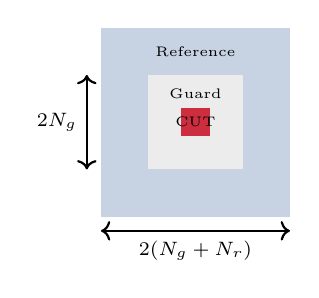
\begin{tikzpicture}[scale=0.6]
    % Outer reference window
    \fill[Atlantic!30] (-2,-2) rectangle (2,2);
    % Guard region
    \fill[Black10] (-1,-1) rectangle (1,1);
    % Cell under test
    \fill[Rose] (-0.3,-0.3) rectangle (0.3,0.3);

    % Labels
    \node at (0,0) {\tiny CUT};
    \node at (0,0.6) {\tiny Guard};
    \node at (0,1.5) {\tiny Reference};

    % Dimensions
    \draw[<->,thick] (-2.3,-1) -- (-2.3,1);
    \node[left] at (-2.3,0) {\scriptsize $2N_g$};
    \draw[<->,thick] (-2,-2.3) -- (2,-2.3);
    \node[below] at (0,-2.3) {\scriptsize $2(N_g+N_r)$};
\end{tikzpicture}
\end{center}

\column{0.48\textwidth}
\textbf{Optimization challenge:}
\begin{itemize}
    \item Parameter space: $N_g \in [1,10]$, $N_r \in [5,30]$, $P_{\mathrm{FA}} \in [10^{-6}, 10^{-2}]$
    \item Noise map depends on $(N_g, N_r)$ only
    \item \alert{Loop hoisting:} compute once per $(N_g, N_r)$, reuse across all $P_{\mathrm{FA}}$
\end{itemize}

\vspace{0.3cm}
\textbf{Speedup factor:} Number of $P_{\mathrm{FA}}$ values tested
\end{columns}
\end{frame}

% Annotation and scoring slide
\begin{frame}{Annotation and Scoring Function}
\small
\begin{columns}[T]
\column{0.48\textwidth}
\textbf{Blob tracing annotation:}
\begin{itemize}
    \item Operator clicks on detected target
    \item 8-connected flood fill captures exact shape
    \item Ground truth blob $\mathcal{B}_k$ = pixel set
\end{itemize}

\vspace{0.3cm}
\textbf{Coverage ratio:}
\begin{equation*}
    \rho_k = \frac{\sum_{p \in \mathcal{B}_k} D_t(p)}{|\mathcal{B}_k|}
\end{equation*}

\vspace{0.3cm}
\textbf{Score mapping:}
\begin{equation*}
    s_k = \begin{cases}
        1.00 & \text{if } 0.8 \le \rho_k \le 1.1 \\
        0.75 & \text{if } 0.6 \le \rho_k < 0.8 \\
        0.50 & \text{if } 0.4 \le \rho_k < 0.6 \\
        0.25 & \text{if } 0.2 \le \rho_k < 0.4 \\
        0.00 & \text{if } \rho_k < 0.2
    \end{cases}
\end{equation*}

\column{0.48\textwidth}
\textbf{Scoring function visualization:}
\begin{center}
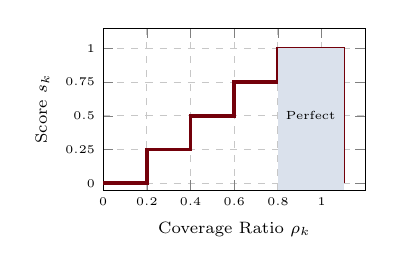
\begin{tikzpicture}[scale=0.85]
    \begin{axis}[
        width=5.5cm,
        height=4cm,
        xlabel={\scriptsize Coverage Ratio $\rho_k$},
        ylabel={\scriptsize Score $s_k$},
        xmin=0, xmax=1.2,
        ymin=-0.05, ymax=1.15,
        xtick={0, 0.2, 0.4, 0.6, 0.8, 1.0},
        ytick={0, 0.25, 0.5, 0.75, 1.0},
        grid=major,
        grid style={dashed, Black30},
        tick label style={font=\tiny},
        label style={font=\scriptsize},
    ]
        \addplot[const plot, color=Garnet, line width=1.5pt] coordinates {
            (0, 0) (0.2, 0.25) (0.4, 0.5) (0.6, 0.75) (0.8, 1.0) (1.1, 0)
        };
        \fill[Atlantic!20] (axis cs:0.8,-0.05) rectangle (axis cs:1.1,1.0);
        \node[font=\tiny] at (axis cs:0.95,0.5) {Perfect};
    \end{axis}
\end{tikzpicture}
\end{center}

\vspace{0.2cm}
\textbf{Frame score (weighted):}
\begin{equation*}
    S_{\mathrm{frame}} = 0.7 \cdot \min_k s_k + 0.3 \cdot \frac{1}{K}\sum_{k=1}^{K} s_k
\end{equation*}
Heavy penalty for missing any target
\end{columns}
\end{frame}

% Grid search algorithm slide
\begin{frame}{Grid Search with Loop Hoisting}
\small
\begin{columns}[T]
\column{0.48\textwidth}
\begin{algorithm}[H]
\scriptsize
\caption{Optimized Grid Search}
\begin{algorithmic}[1]
\STATE \textbf{Input:} frames, blobs, variant
\STATE Pre-compute integral images
\FOR{each $(N_g, N_r)$}
    \STATE Compute noise map $Z$ \alert{← expensive}
    \FOR{each $P_{\mathrm{FA}}$}
        \STATE $\alpha \leftarrow N(P_{\mathrm{FA}}^{-1/N} - 1)$
        \STATE $D_t \leftarrow \mathbb{1}[I_t > \alpha Z]$
        \STATE Score detections vs.\ blobs
    \ENDFOR
\ENDFOR
\STATE \textbf{Return} sorted results
\end{algorithmic}
\end{algorithm}

\vspace{0.2cm}
\textbf{Temporal stability:}
\begin{equation*}
    \mathrm{Stability} = \frac{1}{K}\sum_{k=1}^{K} \frac{c_k}{T}
\end{equation*}
where $c_k$ = frames detecting target $k$

\column{0.48\textwidth}
\textbf{Processing pipeline:}
\begin{center}
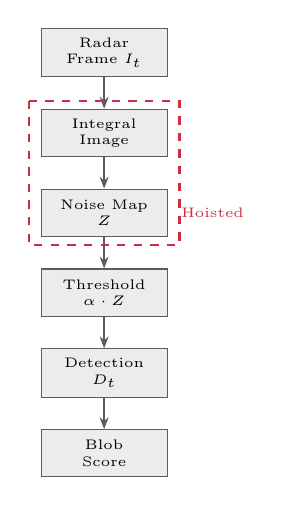
\begin{tikzpicture}[
    block/.style={rectangle, draw=Black70, fill=Black10, minimum height=0.6cm, minimum width=1.6cm, align=center, font=\tiny},
    arrow/.style={-{Stealth[length=1.5mm]}, thick, Black70},
]
    \node[block] (frame) {Radar\\Frame $I_t$};
    \node[block, below=0.4cm of frame] (integral) {Integral\\Image};
    \node[block, below=0.4cm of integral] (noise) {Noise Map\\$Z$};
    \node[block, below=0.4cm of noise] (thresh) {Threshold\\$\alpha \cdot Z$};
    \node[block, below=0.4cm of thresh] (detect) {Detection\\$D_t$};
    \node[block, below=0.4cm of detect] (score) {Blob\\Score};

    \draw[arrow] (frame) -- (integral);
    \draw[arrow] (integral) -- (noise);
    \draw[arrow] (noise) -- (thresh);
    \draw[arrow] (thresh) -- (detect);
    \draw[arrow] (detect) -- (score);

    % Loop hoisting box
    \draw[dashed, Rose, thick] ($(integral.north west)+(-0.15,0.1)$) rectangle ($(noise.south east)+(0.15,-0.1)$);
    \node[font=\tiny, Rose, right=0.05cm of noise] {Hoisted};
\end{tikzpicture}
\end{center}

\vspace{0.2cm}
\textbf{Performance:} $\sim$500 configs in $<$10 seconds
\end{columns}
\end{frame}

% System architecture slide
\begin{frame}{System Architecture: CFAR Studio}
\small
\textbf{Fully client-side web application} -- no installation, no server, no data upload

\vspace{0.3cm}
\begin{columns}[T]
\column{0.48\textwidth}
\textbf{Technology stack:}
\begin{itemize}
    \item React 19 + TypeScript
    \item Vite build system
    \item Plotly.js for interactive visualization
    \item PapaParse for CSV ingestion
    \item Web Worker for grid search
\end{itemize}

\vspace{0.3cm}
\textbf{Key features:}
\begin{itemize}
    \item PPI and B-scan visualization
    \item Multiple colormaps
    \item Interactive blob annotation
    \item Multi-frame temporal analysis
    \item Real-time progress updates
\end{itemize}

\column{0.48\textwidth}
\textbf{Processing pipeline:}
\begin{center}
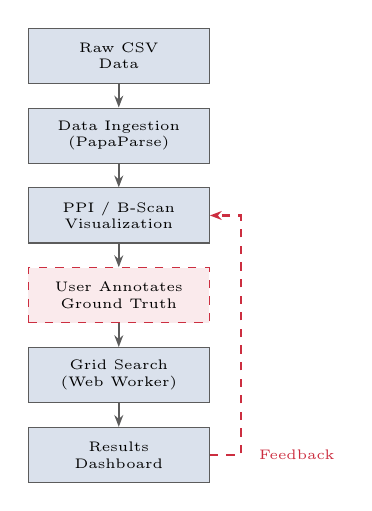
\begin{tikzpicture}[
    block/.style={rectangle, draw=Black70, fill=Atlantic!20, minimum height=0.7cm, minimum width=2.3cm, align=center, font=\tiny},
    userblock/.style={rectangle, draw=Rose, dashed, fill=Rose!10, minimum height=0.7cm, minimum width=2.3cm, align=center, font=\tiny},
    arrow/.style={-{Stealth[length=1.5mm]}, thick, Black70},
]
    \node[block] (csv) {Raw CSV\\Data};
    \node[block, below=0.3cm of csv] (parse) {Data Ingestion\\(PapaParse)};
    \node[block, below=0.3cm of parse] (viz) {PPI / B-Scan\\Visualization};
    \node[userblock, below=0.3cm of viz] (annotate) {User Annotates\\Ground Truth};
    \node[block, below=0.3cm of annotate] (worker) {Grid Search\\(Web Worker)};
    \node[block, below=0.3cm of worker] (results) {Results\\Dashboard};

    \draw[arrow] (csv) -- (parse);
    \draw[arrow] (parse) -- (viz);
    \draw[arrow] (viz) -- (annotate);
    \draw[arrow] (annotate) -- (worker);
    \draw[arrow] (worker) -- (results);
    \draw[arrow, dashed, Rose] (results.east) -- ++(0.4,0) |- (viz.east);
    \node[font=\tiny, Rose, right=0.5cm of results] {Feedback};
\end{tikzpicture}
\end{center}
\end{columns}
\end{frame}

% Results slide 1: PPI with detections
\begin{frame}{Results: PPI View with Detections}
\begin{center}

\includegraphics[width=0.85\textwidth]{figures/ppi_full_view_detections_and_ground_truth.png}
\end{center}
\scriptsize
\textbf{Data:} Furuno DRS4D NXT X-band (9.41 GHz) radar at Lake Murray, SC\\
\textbf{Platform:} Raspberry Pi 5 digitization and recording\\
\textbf{Environment:} Mixed water, shoreline structures, fixed infrastructure
\end{frame}

% Results slide 2: Full UI
\begin{frame}{Results: Full CFAR Studio Interface}
\begin{center}

\includegraphics[width=0.95\textwidth]{figures/full_ui_ppi_with_optimization_results.png}
\end{center}
\scriptsize
Interactive parameter controls (left), PPI display (center), optimization results dashboard (right)
\end{frame}

% Results slide 3: B-scan
\begin{frame}{Results: B-Scan View}
\begin{center}

\includegraphics[width=0.75\textwidth]{figures/bscan_view_grayscale_with_cfar_detections.png}
\end{center}
\scriptsize
Range vs.\ azimuth representation reveals clutter structure and detection behavior along radar spokes
\end{frame}

% Results slide 4: Quantitative findings
\begin{frame}{Results: Optimization Findings}
\small
\textbf{Parameter space:} Grid search over $\sim$500 configurations in $<$10 seconds

\vspace{0.3cm}
\begin{columns}[T]
\column{0.48\textwidth}
\textbf{Guard cells $N_g$:}
\begin{itemize}
    \item $N_g \ge 3$ improves scores for extended targets
    \item Prevents target self-contamination of noise estimate
    \item Point targets less sensitive to guard cell count
\end{itemize}

\vspace{0.3cm}
\textbf{Reference cells $N_r$:}
\begin{itemize}
    \item Optimal range: $N_r \in [10, 20]$
    \item Balance: noise estimation accuracy vs.\ spatial homogeneity
    \item Large $N_r > 25$ degrades performance at terrain transitions
\end{itemize}

\column{0.48\textwidth}
\textbf{False alarm probability $P_{\mathrm{FA}}$:}
\begin{itemize}
    \item Scene-dependent optimal value
    \item Open water: lower $P_{\mathrm{FA}}$ acceptable
    \item Near clutter edges: moderate $P_{\mathrm{FA}}$ maintains detection
\end{itemize}

\vspace{0.3cm}
\textbf{Variant comparison:}
\begin{itemize}
    \item \textbf{GO-CFAR:} fewer false alarms, conservative
    \item \textbf{SO-CFAR:} higher detection, more false alarms
    \item \textbf{CA-CFAR:} best overall in homogeneous scenes
\end{itemize}

\vspace{0.3cm}
\textbf{Temporal stability:} Top configs achieve $>$0.9 across all frames
\end{columns}
\end{frame}

% Discussion and limitations slide
\begin{frame}{Discussion and Limitations}
\small
\begin{columns}[T]
\column{0.48\textwidth}
\textbf{Strengths:}
\begin{itemize}
    \item Formalizes operator knowledge as quantitative objective
    \item Exhaustive search finds scene-specific optimal config
    \item Area-weighted scoring more informative than binary detection
    \item Temporal stability identifies consistent configs
    \item Zero-infrastructure deployment (browser-only)
    \item Open source, no licensing constraints
\end{itemize}

\vspace{0.3cm}
\textbf{Applications:}
\begin{itemize}
    \item Autonomous vessel mapping and deconfliction
    \item Search-and-rescue in cluttered environments
    \item Ad-hoc deployments in unfamiliar scenes
\end{itemize}

\column{0.48\textwidth}
\textbf{Limitations:}
\begin{itemize}
    \item Assumes quasi-stationary targets and fixed platform
    \item Moving targets require frame registration or tracking
    \item Browser constraints: no GPU, single-threaded JS
    \item Practical CSV file size limit: $\sim$50 MB
    \item Grid search feasible for current 3-parameter space
    \item More variants (OS-CFAR) would benefit from Bayesian optimization
\end{itemize}

\vspace{0.3cm}
\textbf{Future work:}
\begin{itemize}
    \item Extend to additional CFAR variants
    \item Support for moving target annotation
    \item GPU acceleration via WebGL/WebGPU
    \item Cross-sensor supervision (e.g., AIS, camera)
\end{itemize}
\end{columns}
\end{frame}

% Questions slide with full Garnet background
{
\setbeamercolor{background canvas}{bg=Garnet}
\begin{frame}[plain]
    \vspace{2.5cm}
    \begin{center}
        {\color{white}\Huge Questions?}

        \vspace{1.5cm}
        {\color{Black10}\Large Human-Supervised CFAR Autotuning\\for Maritime Sensing}

        \vspace{1cm}
        {\color{Black10}\large N. Kirk, J.C. Vaught, D. Cahl, Y. Wang}

        \vspace{0.5cm}
        {\color{Black10}University of South Carolina}
    \end{center}
\end{frame}
}

\end{document}
